\documentclass[
12pt,
english,
ngerman,
headsepline,
twoside,
openright,
numbers=noenddot,version=first
]{scrreprt}

\usepackage{lmodern}
\renewcommand{\sfdefault}{lmss}
\renewcommand{\ttdefault}{lmtt}
\usepackage[T1]{fontenc}
\usepackage[utf8]{inputenc}
\usepackage{listings}
\usepackage[a4paper]{geometry}
\geometry{verbose,tmargin=3cm,bmargin=3cm,lmargin=3cm,rmargin=2.75cm,headheight=1cm,headsep=0.666cm,footskip=1cm}
\setcounter{secnumdepth}{3}
\setcounter{tocdepth}{3}
\setlength{\parskip}{\medskipamount}
\setlength{\parindent}{0pt}

\usepackage{babel}

%% include jabref file
\usepackage{caption}
\usepackage{cite}
\usepackage{courier}
\usepackage{color}
\usepackage{emptypage}
\usepackage[usenames,dvipsnames,svgnames,table]{xcolor}
%\usepackage{listings} doppelt
%\usepackage[printonlyused]{acronym}
%\usepackage{svg}
\usepackage[acronym]{glossaries}
\usepackage{verbatim}
\usepackage{url}
\usepackage{graphicx}
\usepackage{setspace}
\usepackage{float}
\usepackage{graphicx}
\usepackage{subcaption}
\usepackage{color}
\usepackage{csquotes}
\usepackage{totcount}
\usepackage{csvsimple}
\usepackage{amsmath}
\usepackage{rotating}
\usepackage{adjustbox}
\usepackage{tabulary}
\usepackage{lscape}
\usepackage[nomargin,inline,marginclue,draft]{fixme}
\usepackage{wrapfig}
%\usepackage{minted}
%\usepackage{fontspec}

\regtotcounter{chapter}

\setstretch{1.4}
\usepackage[unicode=true,
bookmarks=true,bookmarksnumbered=false,bookmarksopen=true,bookmarksopenlevel=2,
breaklinks=false,pdfborder={0 0 0},backref=false,colorlinks=false]
{hyperref}
\hypersetup{pdftitle={SAKWA},
pdfauthor={Dragoljub Milasinovic}}

\makeatletter

% custom colors
\definecolor{lightergray}{gray}{0.95}
\definecolor{lighterergray}{gray}{0.98}

\DeclareCaptionFont{darkgray}{\color{darkgray}}
\DeclareCaptionFont{black}{\color{black}}
\DeclareCaptionFormat{listing}{\colorbox{lightergray}{\parbox{\textwidth}{#1#2#3}}}
\captionsetup[lstlisting]{
font=sf
,format=listing
,margin=0pt
,labelfont=darkgray
,textfont=black}

\lstset{
basicstyle=\scriptsize\ttfamily,
tabsize=2,
extendedchars=true,
breaklines=true,
frame=bt,
framesep=4pt,
keywordstyle=\color{blue}\ttfamily,
%keywordstyle=\color{violet}\bfseries,
stringstyle=\color{red}\ttfamily,
%stringstyle=\color{black}\ttfamily,
commentstyle=\color{ForestGreen}\ttfamily,
%commentstyle=\color{darkgray},
rulecolor=\color{lightergray},
backgroundcolor=\color{lighterergray},
showspaces=false,
showtabs=false,
xleftmargin=17pt,
numbersep=5pt,
numberstyle=\tiny,
numbers=left,
resetmargins=true,
framexleftmargin=17pt,
framexrightmargin=6pt,
framexbottommargin=4pt,
showstringspaces=false,
morekeywords={__global__},
columns=flexible
}

\lstloadlanguages{
Java, Bash, C++
}

% create css listing style
\lstdefinelanguage{JavaScript}{
keywords={typeof, new, true, false, catch, function, return, null, catch, switch, var, if, in, while, do, else, case, break},
keywordstyle=\color{blue}\bfseries,
ndkeywords={class, export, boolean, throw, implements, import, this},
ndkeywordstyle=\color{darkgray}\bfseries,
identifierstyle=\color{black},
sensitive=false,
comment=[l]{//},
morecomment=[s]{/*}{*/},
commentstyle=\color{black}\ttfamily,
stringstyle=\color{black}\ttfamily,
morestring=[b]',
morestring=[b]"
}

% create css listing style
\lstdefinelanguage{Groovy}{
keywords={as, assert, break, case, catch ,class,const,continue,def,default,do,else,enum,extends
,false,finally,for,goto,if,implements,import,in,instanceof,interface,new,null,package,return,super
,switch,this,throw,throws,trait,true,try,while},
keywordstyle=\color{Black}\bfseries,
ndkeywords={shadowJar, class, boolean, throw, implements, import, this},
ndkeywordstyle=\color{darkgray}\bfseries,
identifierstyle=\color{black},
sensitive=false,
comment=[l]{//},
morecomment=[s]{/*}{*/},
commentstyle=\color{purple}\ttfamily,
stringstyle=\color{gray}\ttfamily,
morestring=[b]',
morestring=[b]"
}


\newcommand{\qq}{\symbol{34}} % 34 is the decimal ascii code for "
\newcommand\invisiblesection[1]{%
\refstepcounter{section}%
\addcontentsline{toc}{section}{\protect\numberline{\thesection}#1}%
\sectionmark{#1}}


%%%%%%%%%%%%%%%%%%%%%%%%%%%%%% LyX specific LaTeX commands.
\providecommand{\LyX}{L\kern-.1667em\lower.25em\hbox{Y}\kern-.125emX\@}
%% Because html converters don't know tabularnewline
\providecommand{\tabularnewline}{\\}

%%%%%%%%%%%%%%%%%%%%%%%%%%%%%% Textclass specific LaTeX commands.
\newenvironment{lyxcode}
{\par\begin{list}{}{
\setlength{\rightmargin}{\leftmargin}
\setlength{\listparindent}{0pt}% needed for AMS classes
\raggedright
\setlength{\itemsep}{0pt}
\setlength{\parsep}{0pt}
\normalfont\ttfamily}%
\item[]}
{\end{list}}

%%%%%%%%%%%%%%%%%%%%%%%%%%%%%% User specified LaTeX commands.
%% Flexibles Seitenlayout
\usepackage[automark]{scrpage2}

%% Mehrspaltenlayout ermöglichen
\usepackage{multicol}

%% Unterstützung für Farben
\usepackage{color}

%% Schönere Tabellen
\usepackage{booktabs, longtable}

%% Schönerer Blocksatz
\usepackage{microtype}


%% Mehr Platz zwischen Überschrift und Tabelle
\newcommand{\@ldtable}{}
\let\@ldtable\table
\renewcommand{\table}{ %
\setlength{\@tempdima}{\abovecaptionskip} %
\setlength{\abovecaptionskip}{\belowcaptionskip} %
\setlength{\belowcaptionskip}{\@tempdima} %
\@ldtable %
}

%% Verschiedene Symbole und Zeichen wie (c)
\usepackage{textcomp}

%% Deutsche Kurzfassung und englisches Abstract auf eine Seite
\renewenvironment{abstract}{
\@beginparpenalty\@lowpenalty
\begin{center}
\normalfont\sectfont\nobreak\abstractname
\end{center}
\@endparpenalty\@M
}{
\par
}

%% Alle Seiten vor dem Inhaltsverzeichnis sind römisch nummeriert
\pagenumbering{roman}
\let\myTOC\tableofcontents
\renewcommand\tableofcontents{
\begin{spacing}{1.1}
\myTOC
\end{spacing}
\clearpage
\pagenumbering{arabic}
}

%% Kopfzeile um Logo ergänzen
\clearscrheadfoot
\ohead{\\\headmark}
\ihead{
\includegraphics[scale=0.4]{pics/2015_10_05_THB_Logo_BW}}%\pagemark}
\ofoot[\pagemark]{\pagemark}

%% Randnotizen anpassen
%\setlength{\marginparwidth}{22mm}
%\let \oldmarginpar = \marginpar
%\renewcommand{\marginpar}[1]{%
%    \-\oldmarginpar[\raggedleft\footnotesize\sf #1]%
%        {\raggedright\footnotesize\sf #1%
%    }}

%% Zitate am Kapitelanfang
\usepackage{epigraph}
\setlength{\epigraphwidth}{9cm}

\makeatother

%-----------------------
%  Glossar https://www.sharelatex.com/learn/
%-----------------------
\makeglossaries


\begin{document}
\titlepage

\begin{center}

\includegraphics[width=12cm]{pics/2015_10_05_THB_Logo_CMYK_randlos}\vspace{0.5cm}

\par\end{center}

\vspace{1cm}

\noindent \begin{center}
\textsf{\textbf{\large BACHELORARBEIT}}\textsf{}\\

\textsf{}\\
\textsf{\huge Serverless / Serverlose Architekturen für Konventionelle Webanwendungen}
\par\end{center}{\Large \par}

\vspace{2cm}

\noindent \begin{center}
{\huge }\begin{tabular}{rl}
Vorgelegt von: & Dragoljub Milasinovic\tabularnewline
Matrikelnummer: & 20140076\tabularnewline
am: & XX. Monat XXXX\tabularnewline
\end{tabular}
\par\end{center}{\huge \par}

\vspace{1cm}

\noindent \begin{center}
zum \\
Erlangen des akademischen Grades\textsf{}\\
\par\end{center}
\noindent \begin{center}
\textsf{\textbf{\large BACHELOR OF SCIENCE}}\textsf{\textbf{\LARGE }}\\
\textsf{\textbf{(B.Sc.)}}
\par\end{center}

\vspace{1cm}

\noindent \begin{center}
\medskip{}
\begin{tabular}{rl}
Erstbetreuer: & Prof. Dr.-Ing. Schafföner\tabularnewline
Zweitbetreuer: & Jonas Brüstel, M.Sc.\tabularnewline
\end{tabular}
\par\end{center}

\noindent \begin{center}
{\huge }
\par\end{center}{\huge \par}

\newpage{}

\selectlanguage{ngerman}%
\tableofcontents{}

\pagestyle{scrheadings}

\chapter*{Eidesstattliche Erklärung}

Ich versichere hiermit, dass ich die von mir eingereichte Masterarbeit selbstständig verfasst, ausschließlich die angegebenen Hilfsmittel benutzt und sowohl wörtliche, als auch sinngemäße entlehnte Stellen als solche kenntlich gemacht habe. Die Arbeit hat in gleicher oder ähnlicher Form noch keiner anderen Prüfungsbehörde vorgelegen.

Brandenburg an der Havel, 21. September 2017

\vspace{3cm}

Dragoljub Milasinovic

\chapter*{Abstrakt}
Pomodoro
@Deutch
@English

\chapter{Einleitung}{Idee-Ausführung-Markt}
\setcounter{page}{1}
\label{chap:introduction}
%\epigraph{\textit{\textquotedbl{}
%An idea is not a mockup\\
%A mockup is not a prototype\\
%A prototype is not a program\\
%A program is not a product\\
%A product is not a business\\
%nd a business is not profits.\textquotedbl{}}}{
%Balaji S. Srinivasan }

%Die vorantreibende Aspekte solcher Handlungsplan sind die Ausführung/Umsetzung der Idee %bis zum Produkt und derer Beziehung zum Markt. Deren Details sind jedoch unbekannt und %variabel.

Die Faktoren am Anfang einer technologischen Umsetzung einer Idee sind:
\begin{itemize}
\item Prof of Concept\label{aspect:proofConcept}
\item Time-To-Market\label{aspect:timeToMarket}
\item Cost of Human Resources:: Skill-shortage\label{aspect:CostHumanResources}
\item Technical technological details\label{aspect:techDetails}
\item Profitability\label{aspect:profit}
\end{itemize}


\section{Motivation}
Auf dem Weg zur technologischen Umsetzung einer neuen Idee liegen unbekannte Schwierigkeiten
bei der Entscheidungen über deren Umsetzung hinsichtlich auf den Architekturentwurf, die IT Infrastruktur, die Drittanbieter von Software, der Auswahl der Infrastruktur usw.
Schwierigkeiten die von spezialisierten Kompetenzen, Fertigkeiten und \glqq Know-How\grqq\ bedürfen.
Gehören jedoch nicht immer zum Problem des Domäns der Anwendung.

\newacronym{FaaS}{FaaS}{Function as a Service}
Für dieses Problem wurde \acrlong{FaaS}, kürz \acrshort{FaaS}\ref{sec:faas}, als Lösung unter der Rubrik \glqq\ Serverless\ref{sec:serverless}\grqq\ von den Hauptanbieter von \glqq Cloud\grqq\ Technologien vorgestellt.

Der Begriff Serverless weist darauf hin, dass die Verwaltung der darunter liegende Serverinfrastruktur von Cloudanbieter übernommen wird. Jedoch begränzt \acrshort{FaaS} dessen Bedeutung durch die Definition des Programmiermodells, nämlich eine Funktion, oder auch \glqq\ Nano-Microservice\grqq.

\newacronym{KOMA}{KOMA}{Kompetenz Matrix}
Im Rahmen des Cloud-Computing handelt es sich in dieser Arbeit um eine Untersuchung der Serverless Architekturen am Beispiel einer Konventionellen Webanwendung. Dabei wird besonders geachtet ob und wie solche Technologien die Umsetzung erleichtern. Die Entwurfsmuster und die Kernfunktionalität werden mit ausschließlich Serverless Technologien am Beispiel von \acrfull{KOMA}, kurz \acrshort{KOMA}\ref{sec:KOMA}, mit AWS umgesetzt.


\section{Ziel}
\label{sec:task}
\newacronym{MVP}{Mivip}{Minimal Viable Product}
\newacronym{SPA}{SPA}{Single Page Application}
Das Ziel ist ein \acrfull{MVP}, kürz \acrshort{MVP}, in Form von einer \acrfull{SPA}, kürz \acrshort{SPA}\ref{sec:spa}, mit ausschließlich Serverless Technologien vor zur Verfügung zu stellen.

Nach der Umsetzung werden die Erfahrungen und Ergebnisse ausgewertet, um dem Leser bei dem Entscheidungsprozess bei der Umsetzung einer Webanwendung besser zu Informieren.

Die Webanwendung soll möglichst für zukünftige Änderungen flexibel sein.

\section{Aufbau der Arbeit}
\label{sec:layout}

Zuerst wird den Leser in die Klassischen Service Modellen\ref{chap:service-models} auffrischt. Zunächst werden die technische Anforderungen und die dazugehörige Beispiele des Serverless Ansatzes erläutert.
\newacronym{AWS}{AWS}{Amazon Web Services}
Das nächste Kapitel überblickt die aktuelle Serverless Angebote der größten Cloud Anbietern.
Anschließend trifft der Leser den Kern der Arbeit bei der Analyse und Darstellung von Serverless Architekturen\ref{chap:aws-serverless} fokussiert auf \acrfull{AWS}, kurz \acrshort{AWS}. Darin werden die Serverless\ref{sec:serverless} Architekturen eingeführt, das Programmiermodell vorgestellt und die Entscheidungsprinzipien\ref{par:serverless-principles} erläutert.
Der praktische Teil mit der Umsetzung und Bewertung von der oben genannte Serverless Webanwendung KOMA\ref{sec:KOMA}.
Am Ende wird es darüber diskutiert, welche Trade-offs entstehen und die Zukünftperspektiven von Serveless Technologien.

\chapter{Grundlagen}
\label{chap:principles}
%\epigraph{\textit{\textquotedbl{}
%There are only two hard things in computer science:\\ cache invalidation and naming %things.\textquotedbl{}}}{ Phil Karlton }
\section{Cloud Eigenschaften}
\label{sec:cloud-char}
Als Software Architekt, Entwickler oder Projektmanager es ist wichtig, die spezifische Eigenschaften von Cloudangebote zu verstehen. Je nach Anforderungen und Art der technologischen Umsetzung lässt sich richtige Auswahl von ein Meer von Cloud Dienste schwer zu treffen. 

Die vorliegende Arbeit beschäftigt sich mit dem Serverless Ausschnitt der Cloud Dienste. 

Im allgemein heben sich folgende Eigenschaften bei der Betrachtung von Cloud Angebote.
\begin{itemize}
	\item Probably not in a list. .... but explained narrativelly
	\item on-demand self-service
	\item  broad network access
	\item  measured service (pay-per-use)
	\item resource pooling and rapid elasticity
\end{itemize}

Daher können die in der Cloud betreibende Anwendungen folgende Eigenschaften haben: 
\begin{itemize}
	\item Isolated state
	\item Distribution
	\item Elasticity
	\item Automated management
	\item Loose coupling
\end{itemize}

Cloud App Props : Isolated state, Distribution, Elasticity, Automated management, Loose coupling

\section{SOA}
\label{sec:soa}
Service Orientierte Architektur SOA unterlegt die Annahme dass, ein System aus mehreren kleinen, austauschbaren, wiederverwendbaren und entkoppelten Diensten bestehen kann. Stellt eine Menge von Entwurfsprinzipien und Standards für dessen Entwicklung und Integration\cite{cloudEssentials}.

Cloud Computing ist ein Serviceliefermodel in dem Services und Ressourcen von Benutzern Internetweit, wie z.B. bei öffentliche Dienste nach Anfrage, verbraucht werden.

SOA ermöglicht gegenseitiges Datenaustausch zwischen Programmen von unterschiedlichen Anbieter ohne zusätzliche Änderungen an die Services vornehmen zu brauchen. Diese Services sollen unabhängig sein und \glqq standard\grqq\ Schnittstellen haben. 

Im Cloud wird es daher in Services und Servicekomposition zentriert.

\begin{wrapfigure}{i}{0.36\textwidth}
	
\includegraphics[scale=0.5]{./pics/2015_10_05_THB_Logo_BW.eps}
\end{wrapfigure}

\newacronym{DSL}{DSL}{Domain Specific Language}
Microservices und Serverless versuchen die Komplexität der SOA anzusprechen. Beide Ansätze zwingen auf Separation of Concerns, häufige Deployments und Heterogene \acrfull{DSL}, kürz \acrshort{DSL}.


Auf einer Seite Microservices können ihren Zustand und Daten halten und werden mithilfe von \glqq Frameworks\grqq implementiert. Auf der anderen Seite Serverless sind Zustandlos.
ConnectWise\cite{ConnectWise}, Netflix\cite{Netflix} und UNLESS\cite{UNLESS} sind beispiele von Unternehmen die von Serverless Architekturen profitieren.

\section{EDA}
\newacronym{EDA}{EDA}{Event Driven Architecture}

Die Serverless Technologien können durch Benachrichtigungen gestartet werden. Diese \acrfull{EDA} Still, verstärkt die Entkopplung temporäre-weise zwischen Producer/Anfrage und Consumer und ermöglicht eine Asynchrone Verarbeitung, ohne dass Fehler das System zum Absturz bringen.


Es lassen sich folgende Vorteile ersichtlichen:
\begin{itemize}
	\item Wiederverwendung von Services in unterschiedlichen Anwendungen sinkt die Entwicklungskosten und Time-To-Market.
	\item Durch die Standarisierung der Services, ein System kann mit eine Rekonfiguration und ohne Wieder-Entwicklung schnell anpassbar auf die Geschäftliche/Externe Bedürfnisse. Agilität.
	\item Monitoring hilft Fehler zu erkennen und die Leistung zu messen.
	\item Aggregate von Services können Komplexere und Domän übergreifende Aufgaben ausführen.
\end{itemize}
\newacronym{REST}{REST}{REpresentational State Transfer}
Im späteren Kapitel tritt REST als teil der \acrshort{EDA} Architekturstil.


\chapter{Klassische Service-Modellen}
\label{chap:service-models}


\section{IaaS}
\label{sec:iaas}
\newacronym{IaaS}{IaaS}{Infrastructure as a Service}
\acrfull{IaaS}, kurz \acrshort{IaaS}, kann als ein Service beschrieben werden, dass Abstraktionen für Hardware, Servers und Netzwerk Komponenten bereitstellt. Der Serviceanbieter besitzt the Ausrüstung und ist für die Behausung, die Inbetriebnahme und die Wartung verantwortlich\cite{patternAWS}. Der Benutzer bezahlt nicht für das Hardware, dessen Lagerung und den Zugang auf ihn, sondern für die Nutzung des gesamtes Servicemodel z.B.: Zahlung nach benutzte Stunden, Ressourcen usw.

\section{PaaS}
\label{sec:paas}
\newacronym{PaaS}{PaaS}{Platform as a Service}
\acrfull{PaaS}, kurz \acrshort{PaaS}, kann als ein Service beschrieben werden, dass eine Rechenplatform liefert, z.B. ein Betriebssystem, eine Ausführungsumgebung für Programmiersprachen(siehe ElasticBeanstalk), eine Datenbank oder ein Webserver. Dieser Dienst übernimmt sowohl die Wartung der Datenbank, Webserver und die Versionen des Laufzeitquellcodes als auch dessen Skalierbarkeit die nun nur Konfiguriert werden bracht\cite{patternAWS}.

\section{SaaS} 
\label{sec:saas}
\newacronym{SaaS}{SaaS}{Software as a Service}
\acrfull{SaaS}, kurz \acrshort{SaaS}, kann als ein Service beschrieben werden, dass OS-Images mit konfigurierbaren Diensten wie Datenbanke, Webanwendungen usw. Der Nutzer muss die Konfiguration und Deployment nicht lernen, um die Dienste in einen größeren \glqq Stack\grqq\ einzubinden. Die Gebühren sind generell nach benutzte Stunde. 

\newglossaryentry{virtualization}{name={Virtualisation},description={Abstraktion der Anwendung, OS oder DB von der darunterliegende Infrastruktur z.B. ein Server.}}

Das \glqq\Gls{virtualization}\grqq\ einer ganzen Umgebung oder Stack zerteilt sich in eine Sammlung von kleinen spezialisierten Aufgaben, die durch Drittanbieter implementiert wurden. Dieser Fakt steigerte die wirtschaftlichen Kosten und machte die Skalierungsmöglichkeiten komplexer\cite{patternAWS}.

\begin{figure}[h]
	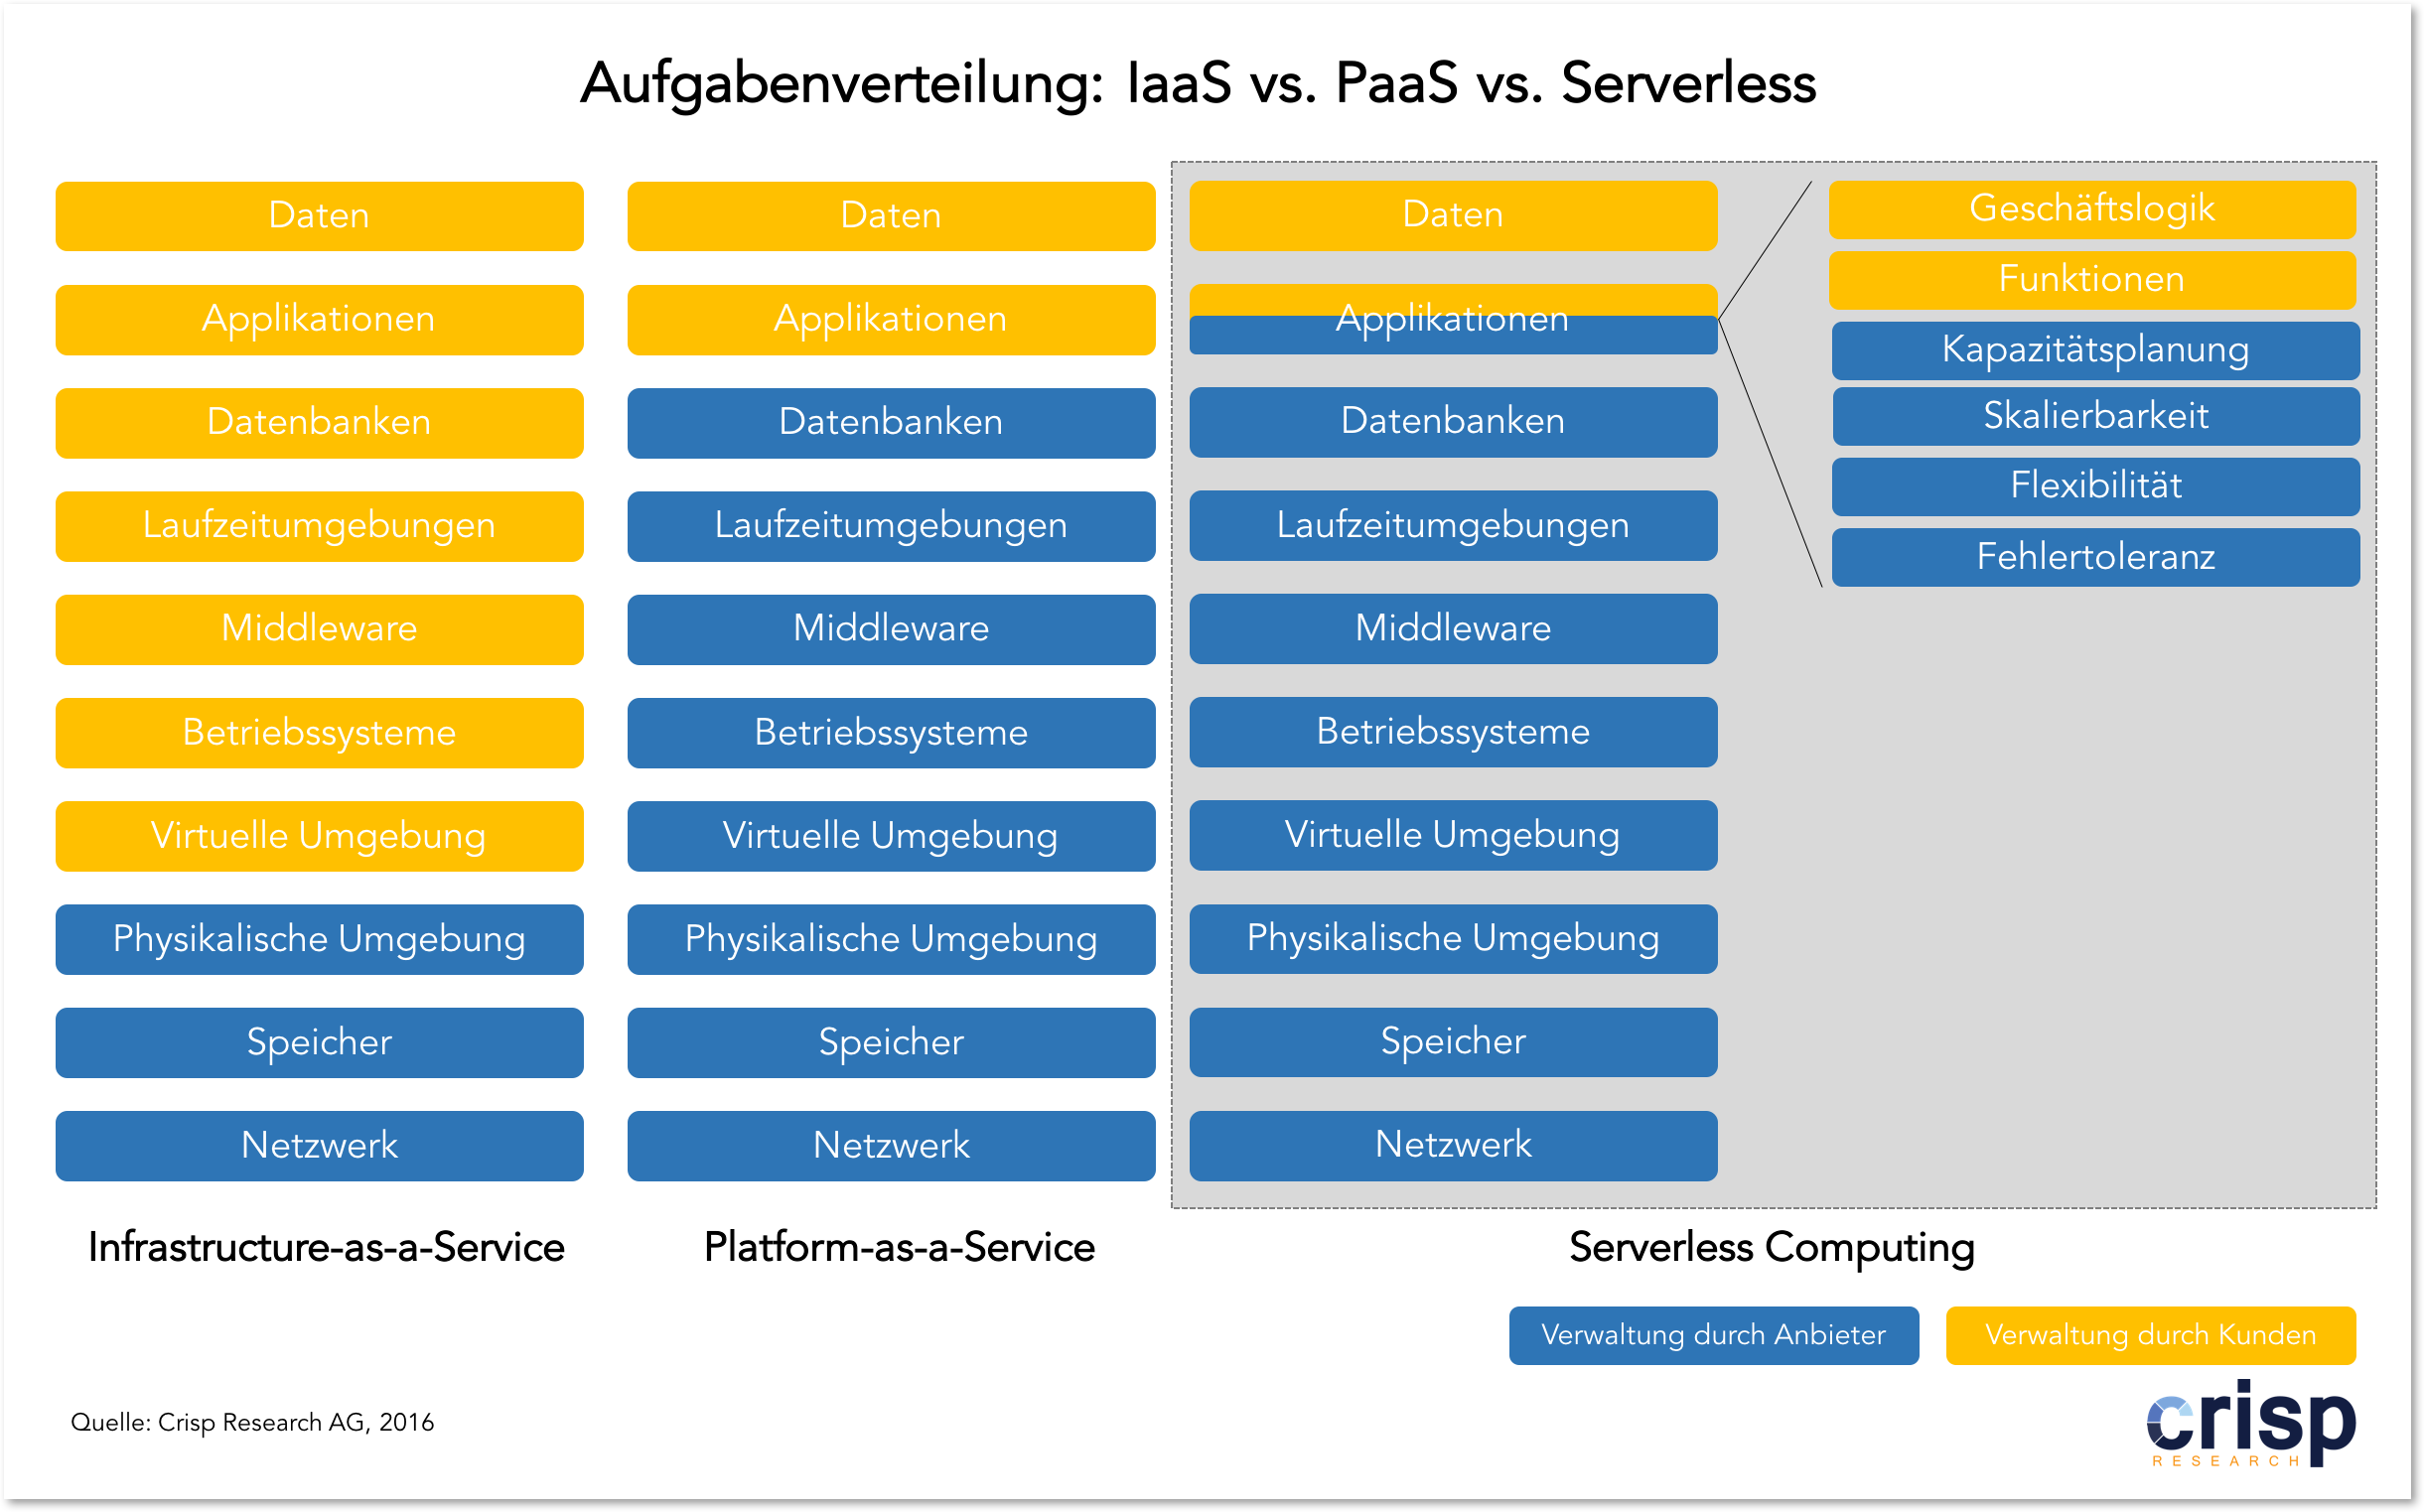
\includegraphics[scale=0.36]{./pics/IaaS_vs_PaaS_vs_Serverless.png}
\end{figure}

\chapter{FaaS}{nichtfunktionalen/technischen Anforderungen zur Entwicklung des Serverless-Ansatzes}

\section{FaaS Definition}
\label{sec:faas}
\acrshort{FaaS} kann als ein Rechen-Service beschrieben werden, dass nach Anfrage isoliert, unabhängig und granular ausgeführt wird. Dessen \glqq Unit of Deployment\grqq\ ist eine Funktion. 

Komplexe Probleme wie horizontale und vertikale Skalierbarkeit, Fehlertoleranz, Flexibilität werden von Kunden und Benutzer nur noch nach bedarf Konfiguriert und von Anbieter verwaltet.

\section{Technische Anforderungen}
Gegenüberstellung 
Skalliebarkeit ok
Vendor-lockin
Customisation
Decentralisation
\section{Ja/Neins}

Die Unterschiede zwischen den\cite{lambdaAWS}
\paragraph{Wann Nicht}: 

Betriebsystemabhängigkeiten erkennen: Traditionellen Computing wie EC2, wo die Entwickler root 
zugrifsrechte auf alle Ressources hat, in Lambda ist diser Opaque.

OS Attribute Konfigurationen: Priorisieren CPU, GPU, Networking, or Disk Speicher und Geschwindigkeit. In Lambda skalieren proportional.

Sicherheit: Lambda nicht sichtbar host-based intrusion detection systems cannot be installed, system-level access logs

Dauerhafte Prozesse. Lambda kann bis 300s. Kosten pro Monat 1Gb  Lambda = 37 EC2 = 9Dollar. Wenn warten auf Requests, oder auf Callbacks geht nicht.

\paragraph{Wann Ja}

EventDriven Tasks: Lambda solves the polling problem by creating an on-demand response to particular events.

Cron. Events: EC2 als behälter von Scripts, kostet auch ohne sie auszuführen. Fehlerhafte Scripts nicht einfach zu erkennen. Skallierung auch von Fehler. Permissions zu offen.
Mit Lambda: the permissions can be much more narrowly applied, failures are much more easily noticed, deployments can be easily triggered, logs are aggregated in one place, and the underlying server management is handled by AWS.

Heavy Processing: Um autoskalling zu vermeiden wegen z.B.Bildverarbeitung. So entkoppelt sich der Empfänger und der Verarbeiter und können mehr Requests angenommen werden. 

Serverless API Gateway vermeidet api servers

Selten verwendete Services. z.B <= 5 porZent average CPU t2.micro <~> 3x10hoch6 = 9dollar

\chapter{wie es sich in die Informatik einbettet}
HTTP, Funktionale Programmierung, Fassaden, ... ?? 
Funktionale programmierung abstrahiert. auf Infrastruktur. ??? 

\section{Use Cases}
next\cite{serverlessArchAWS}
Application Backend: z.b Internet of Things IoT: push to S3, push queue to SQS and invoke Lambda.

Data Procesisng and manipulation: pipeline of :collation and aggregation of data; image resizing;
and format conversion.

Real time processing and analitics: Ingestion of Data -> Kinesis Streams; if Batch size -> Process, Save, Discard -> Lambda

Legacy Api Proxy: Extra RESTful GateWay with lambda on top legacy api. Easier Usage.

Scheduled Services

Bots and Skills

next\cite{lambdaAWS}
Shuttdown untagged EC2 instances. 

Code Deploy

Process inbount mail: 
attachment to S3 + link to it
spam filter

Detect expiring certificates



\chapter{kurzer Überblick über Serverless-Angebote/Architekturen}

\paragraph{Die Architekturentwurfsmuster} helfen uns zu kommunizieren welches Zweck unsere Software erreichen möchte und bieten generische Lösungen für wiederkehrende Probleme bei der Softwareentwicklung.
Wenn eine erfolgreiche Codeänderung von andere Änderung abhängt, soll die Architektur überprüft werden.
Für Konventionelle Webanwendung wird hier damit gehalten, als ein System das über Presentation, Data, and Application/Logik Tiers/Stufe verfügt. Jede Stufe kann mehreren Logik-Layers/Lagen enthalten, die für unterschiedlichen Funktionalitäten des Domäns verantwortlich sind. Logging wäre ein beispiel für Cross-Cutting Concern der Layers hinaus ausspannt. Die Komplexität wächst mit der Beschichtung zusammen.\\


\section{Serverless}
\label{sec:serverless}

\newacronym{API}{API}{Application Interface}
Serverless kann als ein Ansatz, dass  die Verwendung von ein Rechen-Service, Dienste von Drittanbieter, von \acrfull{API}s, kurz \acrshort{API}s und die Anwendung von Architekturmustern( wie ein Front-End, dass direkt mit Services kommunizieren anhand eines \glqq Delegation-Tokens\grqq\ ) fördert, beschrieben werden. \acrshort{FaaS} ist nur ein Aspekt dessen.

\subsection{pipes and filters}
\begin{figure}[H]
	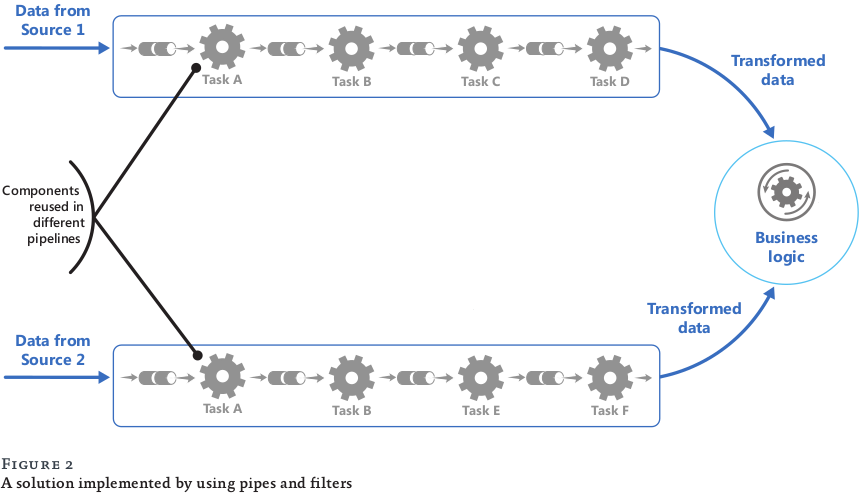
\includegraphics[scale=0.36]{./pics/arch-pipes-filters-sol.png}
\end{figure}

\subsection{compute as a backend}

\begin{figure}[H]
	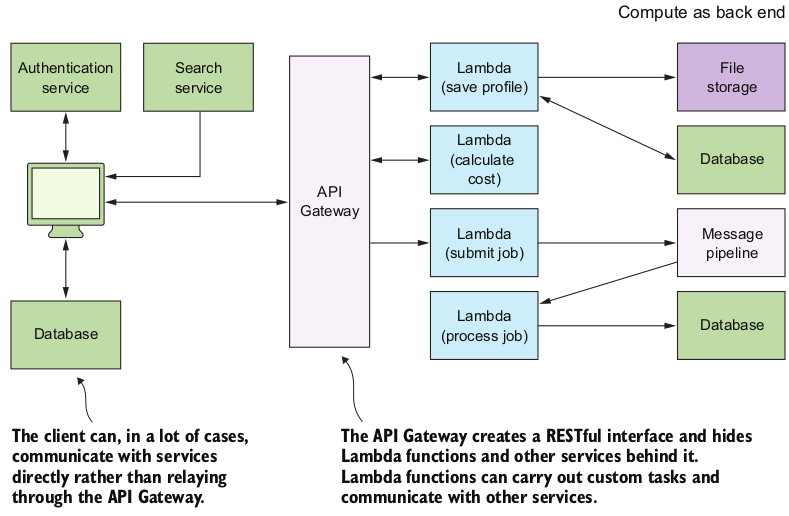
\includegraphics[scale=0.36]{./pics/arch-compute-as-a-backend.png}
\end{figure}


\paragraph{Prinzipien}\label{par:serverless-principles} von Serverless Architeturen: \cite{serverlessArchAWS}
\newacronym{SRP}{SRP}{Single Responsability Principle}
Wie in der Sektion von SOA\ref{sec:soa} erwähnt wurde, das gezwungene Separation of Concerns bring das \acrfull{SRP} mit sich. Funktionen werden dadurch mehr Überprüfbar.
Deren Vernetzung erlaubt komplexe Systeme zu entwerfen, die dank der Stateless Natur der Funktionen schnell zu skalieren sind.
Diese Vernetzung kann durch einen Push-Based Event driven Pipe-line.
Um die Komplexität des Systems zu reduzieren und die längerfristige Wartbarkeit zu verbessern, wird der Controller und/oder Router im Client und Third Party Dienste hinzugefügt.

In einem beispielhaften konventionellen AdServer, nach einem Click auf eine Werbung wird eine Nachricht über ein Kanal an einen Clickprozessor, derer Laufzeit eine Anwendung ist, geschickt. Im Serverless wird dieser Clickprozessor als Funktion pro Nachricht instantiiert derer Laufzeitumgebung und Messagebroker der Cloudanbieter liefert.@Cite Flower's Blog


\section{Technologien}
Microsoft Azure Funktions 
AuthO : AuthO
Firebase : Google
Stack Driver Logging : Google
Cloud Machine Learning Engine : Google
Cloud DataFlow : Google -> Stream batch pipelines
Big Query : Google



\section{Patterns Allgemein vs Serverless}

next\cite{serverlessArchAWS}
Compute as a back end for web and mobile 

compute as a glue pipelines built to carry out workflows <-> Async Messag Primer\cite{patternsCloud}

Pipes and Filters\cite{patternsCloud} <-> lambda event driven
Health endpoint monitoring <-> EC2 certificate
Leader election -> TRansaction mngmt S3
Priority Queue
Queue Based Load Leveling -> Not appliable for Lambda Computing Model
Retry ->
Runtime Reconfiguration <-> Api Gateway Zero Downtime on Redploy
Scheduler Agent supervisor -> Not needed if Design to Failure.
Sharding -> Divide DataStore to Scale better -> Dynamo db + S3
Static Content Hosting -> Solved by S3
Throttling -> Scallability of Serverless Solved vs Transaction
Vallet key <-> Auht0

Befehlmuster wird bei Fusekiserver\ref{komponenten:fuseki} als erteiler der Httpanfrage indem die SparQL Abfrage weiterleiten kann. Daher wird ein Pfad haus/hunde und haus/katze zur gleichen Funktion führen.
Dieser kann aber offline gehen, also mehreren priorisierten MessagePattern als Queue vor eine oder mehreren Lambdas zu setzen absichert die Stabilität des Systems und entkoppelt Komponenten @RoundRobin?? BSRN.
Die Verkettung von Funktionen mittels \glqq Pipes\grqq erlaubt die mehrfache Filterung von Daten.

\section{Guidance}
Caching -> Lambda Reads Same source and Process
Compute partitioning -> Lambda per use. solved
Data Consistency -> Embrace Eventual Consistency in Distributed DBs
Data partitioning <-> Sharding 
Instrumentation and Telemetry Guidance -> Errors Handling
Service Metering -> understand future use of services

\chapter{Fokus auf AWS, Vorstellung der AWS-Serverless-Angebote}
\label{chap:aws-serverless}
Per Type: The Company


\paragraph{Lambda}
\begin{wrapfigure}{i}{0.25\textwidth}
	
\includegraphics[width=0.9\linewidth]{./pics/aws/Compute_AWSLambda.eps}
\end{wrapfigure}

\paragraph{API Gateway}
\begin{wrapfigure}{i}{0.25\textwidth}
	
\includegraphics[width=0.9\linewidth]{./pics/aws/MobileServices_AmazonAPIGateway.eps}
\end{wrapfigure}

\paragraph{Simple Notification Service ( SNS )}
Simple Notification Service ( SNS ) : AWS vs Cloud Pub/Sub : Google
\begin{wrapfigure}{i}{0.25\textwidth}
	
\includegraphics[width=0.9\linewidth]{./pics/aws/Messaging_AmazonSNS.eps}
\end{wrapfigure}

\paragraph{Simple Storage Service ( S3 ) : AWS vs Cloud Storage : Google}
\begin{wrapfigure}{i}{0.25\textwidth}
	
\includegraphics[width=0.9\linewidth]{./pics/aws/Storage_AmazonS3.eps}
\end{wrapfigure}

\paragraph{Simple Queue Service ( SQS ) : AWS }
\begin{wrapfigure}{i}{0.25\textwidth}
	
\includegraphics[width=0.9\linewidth]{./pics/aws/Messaging_AmazonSQS.eps}
\end{wrapfigure}

\paragraph{Simple Email Service ( SES ) : AWS }
\begin{wrapfigure}{i}{0.25\textwidth}
	
\includegraphics[width=0.9\linewidth]{./pics/aws/Messaging_AmazonSES.eps}
\end{wrapfigure}

\paragraph{Relational Database Service ( RDS ) : AWS  }
\begin{wrapfigure}{i}{0.25\textwidth}
	
\includegraphics[width=0.9\linewidth]{./pics/aws/Database_AmazonRDS.eps}
\end{wrapfigure}


\paragraph{DynamoDb}
\begin{wrapfigure}{i}{0.25\textwidth}
	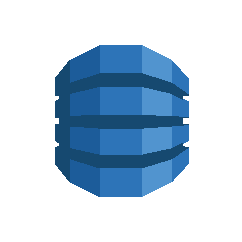
\includegraphics[width=0.9\linewidth]{./pics/aws/Database_AmazonDynamoDB.eps}
\end{wrapfigure}

\paragraph{CloudSearch}
\begin{wrapfigure}{i}{0.25\textwidth}
	
\includegraphics[width=0.9\linewidth]{./pics/aws/Analytics_GRAYSCALE_AmazonCloudSearch.eps}
\end{wrapfigure}

\paragraph{CloudFront ( CDN )}
\begin{wrapfigure}{i}{0.25\textwidth}
	
\includegraphics[width=0.9\linewidth]{./pics/aws/NetworkingContentDelivery_GRAYSCALE_AmazonCloudFront.eps}
\end{wrapfigure}

\paragraph{DNS management ( Route 53 )}
\begin{wrapfigure}{i}{0.25\textwidth}
	
\includegraphics[width=0.9\linewidth]{./pics/aws/NetworkingContentDelivery_AmazonRoute53.eps}
\end{wrapfigure}

\paragraph{Caching (ElastiCache)}
\begin{wrapfigure}{i}{0.25\textwidth}
	
\includegraphics[width=0.9\linewidth]{./pics/aws/Database_GRAYSCALE_AmazonElasticCache.eps}
\end{wrapfigure}

\paragraph{Elastic Transcoder}
\begin{wrapfigure}{i}{0.25\textwidth}
	
\includegraphics[width=0.9\linewidth]{./pics/aws/ApplicationServices_GRAYSCALE_AmazonElasticTranscoder.eps}
\end{wrapfigure}


\paragraph{Kinesis Streams}
\begin{wrapfigure}{i}{0.25\textwidth}
	
\includegraphics[width=0.9\linewidth]{./pics/aws/Analytics_AmazonKinesis.eps}
\end{wrapfigure}

\paragraph{Cognito}
\begin{wrapfigure}{i}{0.25\textwidth}
	
\includegraphics[width=0.9\linewidth]{./pics/aws/MobileServices_GRAYSCALE_AmazonCognito.eps}
\end{wrapfigure}


\chapter{Beispiel(!)-Fall KOMA}

\section{Anforderungen Analyse}

Zu den Anforderungen
\begin{itemize}
	\item Mit dem EQF vergleichbare Kompetenzeindefinitionen
	\item Von Browser abrufbar
	\item Private Datenspeicherung u.d Login
	\item Zukünftige Erweiterungen berücksichtigen
	\item Ertrag von großen Nutzlastschwankungen
\end{itemize}


\section{KOMA}{Beispiel Anwendung}
\label{sec:KOMA}
\newacronym{EQF}{EQF}{European Qualifications Framework}
Die Beschleunigung der Veränderungen in der Heutigen Gesellschaft und dem technologischen Horizont prägt sich sowohl in Bildung als auch in Beruf in so fern aus, dass die heutige Rahmenlehrpläne nicht mehr fachlich sondern nach Kompetenzentwicklung orientiert sind, um Kompetenzprofile für Lerner zu gestallten. Es existiert bereits ein anerkanntes Europäisches Rahmen für Kompetenzbildung: \acrfull{EQF}. Am Beispiel von Sachsen-Anhalt\cite{BildungsServerSachsen} wird diese Kompetenzorientierung auf die spezifische Bedürfnisse der Schule beschrieben und die Untertischstunden entsprechend gestaltet.

Die Umsetzung der Anwendung soll auf einer Seite die von einem Individuum oder Schüler
erworbene und zu erwerbenden Kompetenzen und deren Niveau nachvollziehen. Und auf der Anderen die entsprechende Bildungs-, Unterrichts- und Stundenplanung unterstützen.
Der Kompetenzstand einer Person ist mit dem \acrshort{EQF} vergleichbar, und daher International anerkennbar.

%Diese soll für die pädagogische Diagnostik und Intervention genutzt werden.
Wenn diese Anwendung in Bildungsinstitutionen eingesetzt wird, dienen die Rahmenlehrpläne als Leitpfad für die Belegung der Kompetenzen und \acrshort{KOMA} für die Organisation der einzelnen Fachrichtungen oder Lehrveranstaltungen. 

Der Kern solcher Organisation ist die Zuweisung von Aktivitäten auf vordefinierten Kompetenzen. Aktivitäten lassen sich einzeln oder in einer Sequenz anordnen. Sequenzen werden in Lehrveranstaltungen zusammengestellt. So können Aktivitäten, Sequenzen und Kompetenzen
als Gestaltungsmittel für Lehrveranstaltungen benutzt. Das Modell verfügt von eine Figur um die erledigte Aktivitäten auszuwerten, nämlich Evaluation.

\paragraph{Bild des Modells}
\begin{figure}
	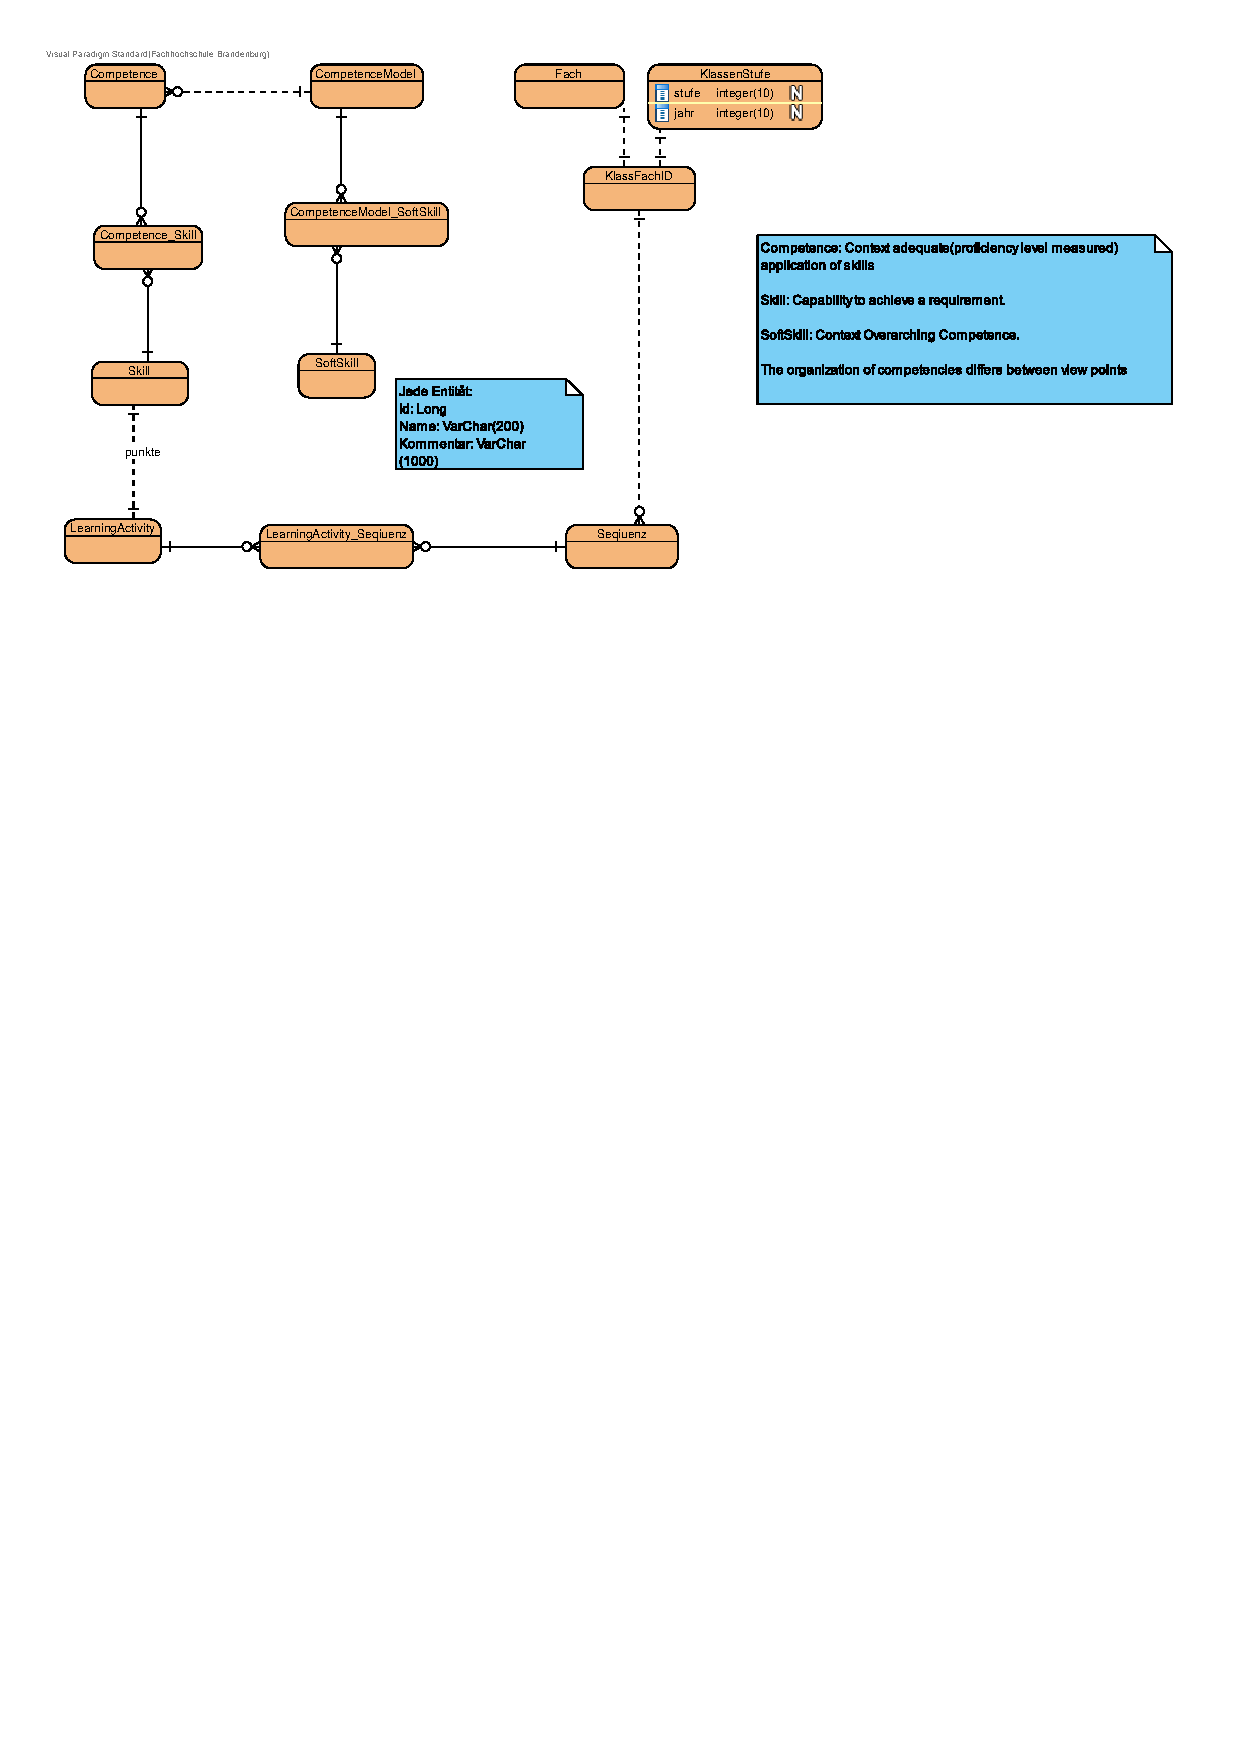
\includegraphics[scale=0.5]{./pics/koma-er-physical.pdf}
\end{figure}

\paragraph{Bekannte Beispiele}

\chapter{Entwurf}
\label{chap:design}

\chapter{Umsetzung}
\label{chap:impl}
Die grundlegende Vorgehensweise bei der Umsetzung dieses Projekts wird Analyse, Entwurf, Implementierung und Test sein. Der Forschender Charakter dieses Projekts lässt sich nicht Testgetrieben implementieren.
Das


\section{Komponenten Übersicht}
\label{sec:components}
Um dem Leser einen Anhaltspunkt zu verleihen, werden hier die Softwarekomponenten beschrieben.

\begin{figure}[H]
	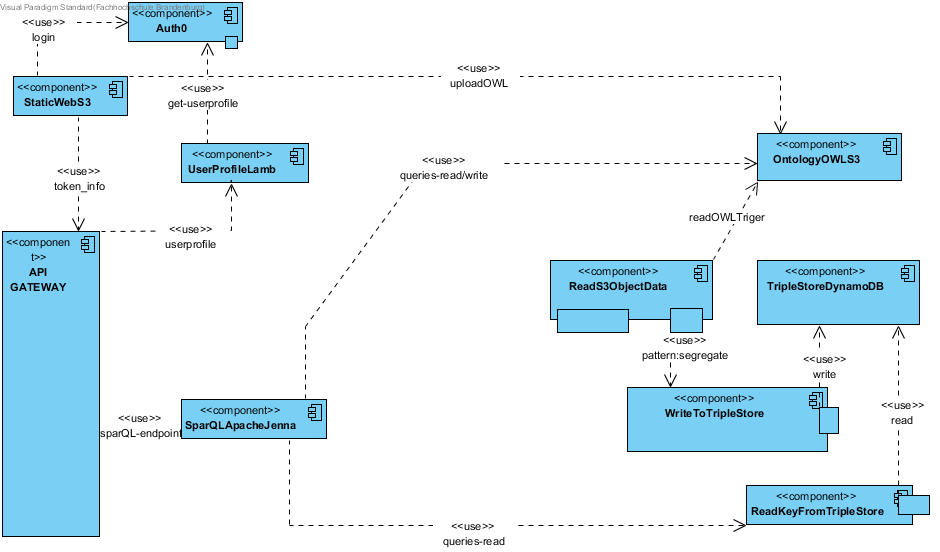
\includegraphics[width=\linewidth]{pics/arch-comp.png}
\end{figure}

legacy api proxy\cite{serverlessArchAWS}
lambda<convert/invoke> fuseki-server\label{komponenten:fuseki}

nice: graphQL= json matcher over multiple DBs




\section{Datenhaltung Analyse und Auswahl}

Die Gestaltung von Kompetenzmodellen und deren zukünftige Weiterentwicklung hängt stark von spezifischen Bedürfnisse jeweiliger Schulen ab. Die mögliche Erweiterungen oder Anpassungen des Modells stellt die Benutzung des einer Relationale Datenbank für \acrshort{KOMA} in Frage. Im Folgendem werden die Eigenschaften von relationalen mit ontologischen Schemas verglichen.


%@Pre-Dev--> Tabelle 
\begin{table}[h]
	\caption{Vergleich relationalem mit ontologischem \ref{subsec:ontology} Schema}
	
	\centering{}
	\begin{tabular}{ccc}
		\noalign{\vskip\doublerulesep}
		Eigenschaft & Relational & Ontologisch \tabularnewline[\doublerulesep]
		\hline\noalign{\vskip\doublerulesep}
		Darstellung Welt-Annahme & Existiert nur & Existiert mindestens \tabularnewline[\doublerulesep]
		\noalign{\vskip\doublerulesep}
		Individual & muss Unique & kann >= 1 \tabularnewline[\doublerulesep]
		\noalign{\vskip\doublerulesep}
		Info & Ableitung = x & ja \tabularnewline[\doublerulesep]
		\noalign{\vskip\doublerulesep}
		Oritentation & Data & Bedeutung \tabularnewline[\doublerulesep]
		
	\end{tabular}
\end{table}

Der Fokus auf die Erweiterung und Bedeutung des ontologischen Schemas führt deren Auswahl als Datenhaltungstechnologie. 

Es handelt sich daher um eine \glqq Linked Data Driven Web Application\grqq.%@href 
Dieser Begriff gehört zum \glqq Semantic Web\grqq,der in der Sektion der Ontologie\ref{subsec:ontology} weiter erläutert wird.

\subsection{Semantic Web}

Das \glqq Semantic Web\grqq ist eine Erweiterung des herkömmlichen Web, in der Informationen mit eindeutigen Bedeutungen versehen werden\cite{ontoWhat2}.
set of standards and best practices for sharing data and the semantics of that data over the Web for use by applications\cite{sparqlLearn}.

\newacronym{OWL}{OWL}{Web Ontology Language}
Diese Bedeutungen werden für Maschinen durch Ontologien dargestellt wessen Spezifikation von W3C\cite{W3C} mit dem Nahme \acrfull{OWL} beschrieben wurde.

\begin{figure}[h]
	\centering
	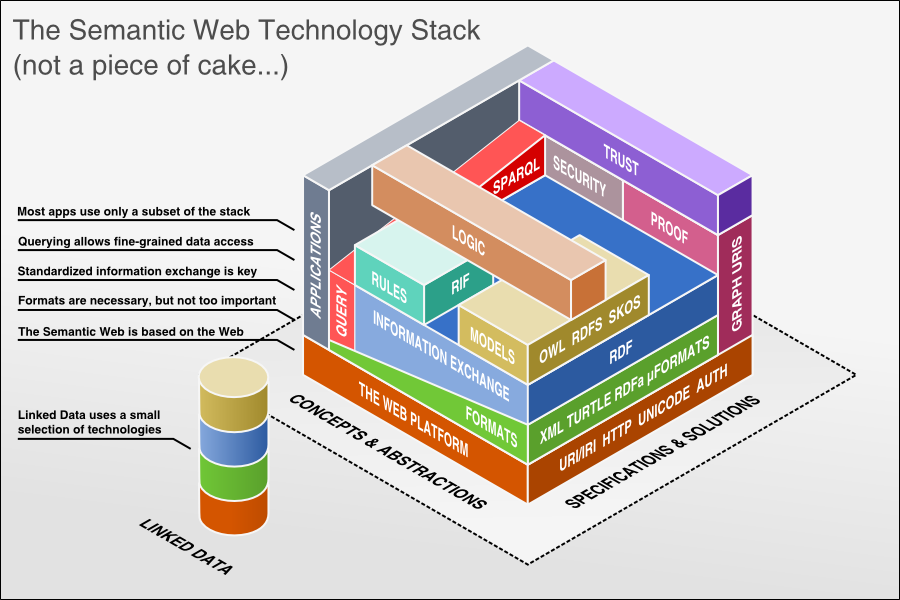
\includegraphics[width=0.8\textwidth]{pics/semantic_web_technology_stack.png}
	\caption{Überblick von benutzten Technologien}
	\label{fig:semantic-web-stack}
\end{figure}

\subsection{Ontologie}{Konzeptuelle Modellierung}
\label{subsec:ontology}

%@Def
Eine Ontologie ist eine formale Spezifikation über eine Konzeptualisierung\cite{ontoWhat}. Die Denotation jeweiliger dargestellten Signifikanten lässt sich durch seinen weltweit eindeutigen Präfix identifizieren. Deren Beziehungen können auch zu externen Ontologie-signifikanten verweisen und dadurch ein Consensus über Begrifflichkeiten. 

Während der Umsetzung wurde Protege\cite{Protégé} benutzt.
Der Entwurf der Ontologie wurde nach Ontology-Engineering-101 durchgeführt:


Um die Neuerfindung des Rades zu vermeiden, die Recherche ergab einen aktuell öffentlichen graphischen ontologischen Entwurf\cite{ontoMoodle} siehe\ref{fig:competence-ontology} der in Moodle mit eine Relationalen Datenbasis und PHP umgesetzt. Nach dessen Ontologien wurde mittels Watson\cite{Watson} und LOD\cite{LOD} nichts öffentlich gefunden. 


\begin{figure}[h]
	\centering
	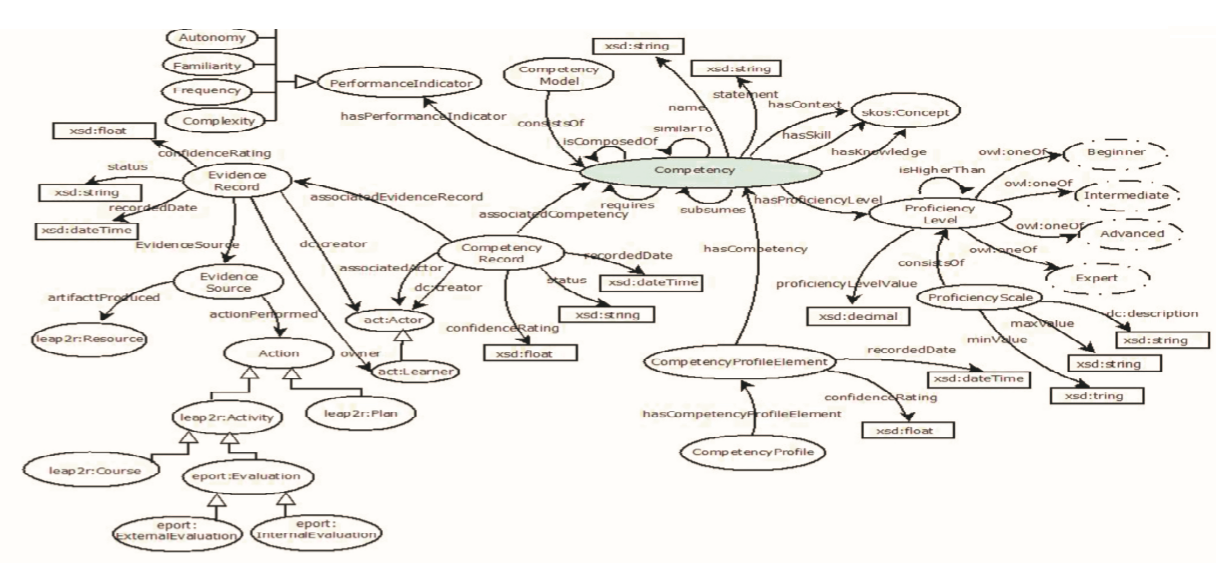
\includegraphics[angle=90]{pics/competency-ontology.png}
	\caption{Kompetenzontologie}
	\label{fig:competence-ontology}
\end{figure}

Bei der Analyse lässt der Entwurf und dessen Dokumentation freie Interpretation über Begriffe und deren Zweck, beispiele davon sind \glqq isComposedOf\grqq, \glqq subsumes\grqq. Ein Standard zur graphischen Darstellung ist zur Zeit?? noch nicht anerkannt. Obwohl Graphische Benutzeroberfläche  @Cite research-gate graphol

Anderseits wurde das \acrshort{EQF} für Ontologien beschrieben, aber nicht öffentlich umgesetzt. Es bietet dabei eine europäisch anerkannte Definition von Kompetenz, nämlich RCD\cite{eqfCompetency}


\begin{wrapfigure}{i}{0.36\textwidth}
	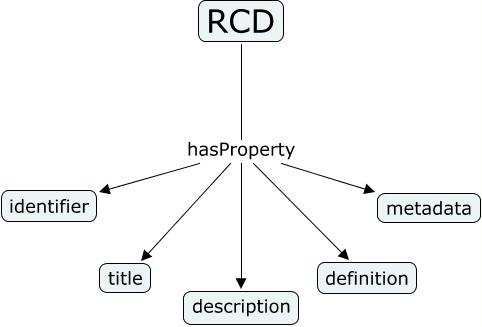
\includegraphics[width=0.9\linewidth]{pics/RCD.jpg}
\end{wrapfigure}


Daher folgt eine beispielhafte Erklärung der auf unseren Anwendungsfall angepasste und ergänzende Interpretation der dargestellten Terminologie des Entwurfs und der RCD.



\newglossaryentry{Kompetenz}{name={Kompetenz},description={die bei Individuen verfügbaren oder durch sie erlernbaren kognitiven Fähigkeiten und Fertigkeiten, um bestimmte Probleme zu lösen, sowie die damit verbundenen motivationalen, volitionalen und sozialen Bereitschaften und Fähigkeiten, um die Problemlösungen in variablen Situationen erfolgreich und verantwortungsvoll nutzen zu können}}

\subparagraph{Erklärung der Terminologie}Die zwei Leitmotive sind auf eine Seite \underline{Kompetenzanforderungen}: sie legen fest, über welche Kompetenzen ein Schüler, eine Schülerin verfügen muss, wenn wichtige Ziele der Schule als erreicht gelten sollen. Systematisch geordnet werden diese Anforderungengen in Kompetenzmodellen, die Aspekte, Abstufungen und Entwicklungsverläufe von Kompetenzen darstellen\cite{competence}. Und auf der Anderen nach \underline{\Gls{Kompetenz}} als die bei Individuen verfügbaren oder durch sie erlernbaren kognitiven Fähigkeiten und Fertigkeiten, um bestimmte Probleme zu lösen, sowie die damit verbundenen motivationalen, volitionalen und sozialen Bereitschaften und Fähigkeiten, um die Problemlösungen in variablen Situationen erfolgreich und verantwortungsvoll nutzen zu können\cite{weinert2002leistungsmessungen}.

\subsection{RDF}
\newacronym{RDF}{RDF}{Resource Description Framework}
\newacronym{TURTLE}{TURTLE}{Terse RDF Triple Language}
Die bisher erreichte Analyse des Domänsproblems soll nun anhand von Protégé in einen \acrfull{RDF} format beschrieben werden. Der Menschen lesbarsten \acrshort{RDF} Format ist \acrfull{TURTLE}. Seine Syntax besteht aus Triples mit \glqq .\grqq beendete Zeilen. Ein Triple stellt ein Fakt dar, un besteht aus einem Subjekt, einem Prätikat und einem Objekt. Diese können sich in TURTLE verschachteln wie das folgende Listing\ref{lst:turtle} zeigt.

\begin{lstlisting}[language=SQL,caption={Darstellung von Triples in TURTLE},label={lst:turtle}]
:EvidenceRecord rdf:type owl:Class .

:actionPerformed rdf:type owl:ObjectProperty ;
rdfs:domain :EvidenceSource ;
rdfs:range :Action .
\end{lstlisting}


\subsection{Sparql}
\newacronym{Sparql}{Sparql}{Protocol And RDF Query Language}
Um aus Ontologien Informationen zu entnehmen, wird die Abfragesprache \acrfull{Sparql} 
verwendet. Diese ist ähnlich zu SQL. Mit dem Programm \glqq Protétegé\grqq können SPARQL Abfragen lokal ausgeführt werden.

Die einfachste Abfrage in Sparql wählt alle Triples vom Datenmodell.

\begin{lstlisting}[language=Sparql]
SELECT * WHERE { ?s ?p ?o .}
\end{lstlisting}

Am Beispiel von KOMA, konkatenieren die Ergebnisse mit Zwei Abfragetriples dank eine Hilfsvariable. Die folgende Abfrage ließe sich \glqq Wähle alle Properties des Graphes und wähle alle dessen Subjekten mit Alice als Objekt\grqq formulieren. \\
\begin{lstlisting}
PREFIX owl: <http://www.w3.org/2002/07/owl#>
PREFIX rdf: <http://www.w3.org/1999/02/22-rdf-syntax-ns#>
PREFIX rdfs: <http://www.w3.org/2000/01/rdf-schema#>
PREFIX koma: <https://s3-us-west-2.amazonaws.com/ontology.thb.de/koma-complex.owl#>
SELECT ?x WHERE {
?y rdf:type owl:ObjectProperty .
?x ?y koma:Alice .
}
\end{lstlisting}

So dass auch die Benutzer von \acrshort{KOMA} solche Abfragen stellen können wird ein \glqq Sparql-endpoint\grqq mit Hilfe von Apache Jena ARQ, ein Sparql-Engine, zur Verfügung gestellt. 
%Fuseki ist ein Server zur Verwaltung von Sparqlabfragen und deren Transaktionen. @Cite CRUD und ACID RDB in sparql.
%Fuseki wird Embedded benutzt.
Dieser Sparql-Endpoint entspricht der Repositoryschicht der Anwendung und wird nach Anfrage von der Ontologie in S3 mittels Sparql JSON Objekte zurückliefern.
Eine Lambdafunktion arbeitet als Schnittstelle \ref{lst:lambda-interface} zwischen die ARQ Bibliothek, den Client und die darunterliegende Infrastruktur.


Um den Datenmodell möglichst simpel programmatisch abzufragen wird zunächst dessen Schnittstelle\ref{sec:rest} definiert. 


\section{Abtrennung des Monoliths}

Im Folgendem es wird beispielhaft eine abtrennung einer JEE Anwendung.

\paragraph{JEE.war}
\glqq And\grqq Test vs SRP
Identifizieren der Concerns und ihre Trennung: 

\subparagraph{Einloggen}
Login beispiel: 
user + password + userData -> 
user + passord -> uuID -> userData 
refactor and share common code


Autorisierung und Authentifizierung. Einleitung

Auth0 bietet Authentifizierung as a Service an. Der Benutzer erhält einen JSON Web Token JWT und schickt ihn Encoded JSON Web Signature JWS oder JSON Web Encription zur Anwendung mit.
%Mit wenige Konfigurationsschritte kann man die Benutzer Authentifizieren. 


Einloggen: 0Auth Google gibt token, der wird in Lambda überprüft, Session in oauth.com verwaltet


\subparagraph{Dynamo DB}

Funtion: Read + Write + updateS3 
zu
Split S3, Split R/W 

Datenspecherung Architektur:
DynamoDB: speichert :individual als Schlussel und seine relative URL
Ś3: speichert die .owl Dateien.

Lambda Funktion: Maps zwischen S3 und DynamoDB.



\section{RESTful API}
\label{sec:rest}
Designing a friendly Hypertext Transfer Protocol (HTTP) API means abstracting the
intricate business logic and data your service uses into the four basic CRUD operations
(create, read, update, delete).

Die Komplexität des darunterliegenden Datenmodells erlaubt eine RESTful\cite{microAdv} Schnittstelle nur einfache abfragen zu formulieren. Daher zusätzlich ein Endpunkt\ref{tab:rest} für Komplexe Sparql Abfragen, die im Body des HTTP Requests in JSON geschickt wird. 

\begin{table}[H]
	\caption{RESTful API}\label{tab:rest}
	\noindent 
	\centering{}
	\begin{tabular}{ccc}
		\hline
		\noalign{\vskip\doublerulesep}
		Methode & URL & Rückgabe\tabularnewline[\doublerulesep]
		\hline
		\noalign{\vskip\doublerulesep}
		GET & /ontology & Information über KOMA
		\tabularnewline[\doublerulesep]\noalign{\vskip\doublerulesep}
		\noalign{\vskip\doublerulesep}
		GET & /ontology/\{individual\} & RDF von Individual
		\tabularnewline[\doublerulesep]\noalign{\vskip\doublerulesep}
		GET & /page & Auflistung von Entitäten 
		\tabularnewline[\doublerulesep]\noalign{\vskip\doublerulesep}
		GET & /page/\{individual\} & Information über diesen Fakt
		\tabularnewline[\doublerulesep]\noalign{\vskip\doublerulesep}
		POST & /sparql & Abfragenergebnis
		
	\end{tabular}
\end{table}

AWS API Gateway ermöglicht die Definition, Konfiguration und das Importieren von Schnittstellen. Beispielsweise kann die Abfrage GET https://<host>/page/\{individual\} 

\begin{lstlisting}[language=Javascript,caption={API Gateway Request Mapping Template},label={lst:map-template}]
GET https://<host>/page/{individual} 
...
{
"individual" : "$input.params('individual')"
}
\end{lstlisting}

Damit wurde die zu erwartende Eingabe für den Sparql-Endpoint definiert. Der Zugang auf die Schnittstelle wird durch CORS konfiguriert um deren Ausnutzung zu vermeiden. 

Dieser Endpunkt unterstützt nicht nur GET-Abrufe, sondern auch POST-Anforderungen mit einer Nutzlast.
Unter der verfügbaren SparQL endpoints Implementierungen



\section{Single Page Application}
\label{sec:spa}

Da KOMA ohne Vorkenntnisse gebrauchsfertig sein soll, mit dem Fakt dass Milliarden von Desktop Geräte die Web mit einem Browser erkundigen können, lässt sich die Entscheidung über die Art der Benutzeroberfläche leicht Treffen.

Die Web Anwendung ist für alle Rechenaufgaben verantwortlich die im Browser aus dem Sicherheitssichtpunkt kein Gefahr darstellen, um den Backend oder Servers möglichst wenig auszulasten. Deswegen bietet sich eine Single Page Application an. 
Die SPA besteht aus ein einziges HTML Dokument. Dies vereinfacht man die Konfiguration der Authentifizierung und unterbricht den Fluss der UI-Darstellung zwischen Seiten.

Ein konfiguriertes Anfangsprojekt/Quickstart kann mithilfe von Initializr\cite{Initializr} oder JHipster\cite{Jhipster}. Für die lokale Entwicklung der Webseite werden anhand von NodeJS und NPM folgende Bibliotheken als Abhängigkeiten verwaltet: Bootstrap als Stylescheet und jQuery als Javascript-Bibliothek.
Die Webseite wird Statisch mittels S3 geliefert. Dies geschieht mit einem Befehl: 
\begin{lstlisting}[language=BASH, caption={Webseite veröffentlichen}]
$ aws  --region us-west-2 s3 website --index-document index.html --error-document error.html 's3://koma.thb.de'
\end{lstlisting} 

Da der Zugriff auf die Datenspeicherung gesichert werden soll, wird die Login-Funktionalität hinzugefügt.


\chapter{Bewertung}

\paragraph{Zur Skalabilität}
Skallabilität in Datenhaltung -> Entwerfe für Distribution + vorteile von Lokalität.
Read replikas -> evtl. Konsistent. 
Viele Perspektiven von Daten -> Lebenszyklus von Daten. 
---- Bounded Context ---- 
Service ist nicht nur Funktion oder nur DB.
Entkopplung fordert enkapsulation und Cohesion.

Event als Bussinesmanager -> Coordinator / Orchestrator -> Lambda
Als Finite State Machine oder WorkFlow

\paragraph{Anwendung}{Latenz}
Die entstandene Webanwendung befindet sich in US-WEST-2, Oregon, in den USA. 
Da keine Cache oder CDN Funktionalität weder Implementiert noch konfiguriert ist, ist die Latenz direkt proportional zur Ausführungsdauer der Lambda Funktion.
@Benchmark testing curl 
@Lambda Monitoring

In Zeiten des Cloud computings 
\paragraph{Frameworks und FaaS}
Frameworks helfen aber sind platform abhängig. Entweder JEE und JVM oder PHP.
Es kann auf die Layer of Abstraction in FW verzichtet werden. 
Die Ersetzbarkeit des FaaS entkoppelt die Anwendung und den Entickler von der darunterliegende Technologie.

\paragraph{DevOps Frameworks}
Die benötigte Fertigkeiten für die Umsetzung einer Serverless Anwendung werden mithilfe von Deploymentframeworks gemindert. Die Aufnahme von 3.Anbieter ist deswegen notwendig. Es existieren bereits solche Hilfe wie z.B Serverlessframework@Ref

Risiko:
Entickler brauchen einen guten Testplan und eine gute DevOps Strategie.<- skills shortage

\paragraph{Transaktionen}
Transaktionen können nicht parallel ausgeführt werden. Sequenciel aka Messaging Pattern.
Zusammenspiel Arch. interfaces prog.modell und FW
Arch 1st -> def interfaces and interactions. to program to a inteface


Eventual consistency -> event driven + ontology quality
Consistenty -> koma-standalone <- transaction mgm

\paragraph{Vorteile}
Automatische Skalierung <!-- größe und kleine Apps --> und Fehlertoleranz
Automatisches Kapazitätsmanagement
Flexible Ressourcenverwaltung
Schnelle Bereitstellung der Ressourcen
Exakte nutzungsabhängige Abrechnung der Ressourcen
Konzentration auf den Kern des Source-Codes


\paragraph{Nachteile}


SLA Service Level Agreement: Latency, Bank:High volume Transactions,
Decentralisation of Services = Challenge = Overhead, time, energy <- orchestration of events.
Decentralisation vs monotithik != --komplexity
Kontrollverlust
Erhöhtes Lock-in Risiko

kurzlebige konfigurationen herausfinden ?? tracking?
viel Konfiguration, kaum Konveniton -> .json 4 everything
local testing braucht event-symulation.json



\paragraph{Zur Entwicklung}
Die Starke Komponentisierung und Dezentralisierung von Software, die Variabilität von Programmiermodellen, Frameworks, Tools, -Sprachen und dessen Entwicklungsumgebung erhöht die Komplexität des Enwicklungscyklus und hervorhebt die Bedürfnis von Tools zur Automatisierung von Tests, Deployment und Konfiguration. Also ein wohldefiniertes Handlungsplan bei der Softwareentwicklung dass von der nicht zu bearbeitende Details abstrahiert. 
Die DevOps Kultur spricht solche Probleme an. Neben dem Entwurf der Softwareachitekture  muss, um derer Umsetzung Zeitgemäß zu gewährleisten, eine zum Projekt passende DevOps Strategie.
Um Vorteil von der neuen Technologien zu nehmen, ist die Recherche nach schon existierenden DevOps Frameworks besonders wichtig. Dessen Integration in der DevOps Strategie diene für eine Agile Entwicklung.

\paragraph{Zum Datenmodel}
Aus der Anforderungs analyse einer Informations Techonologie Web Anwendung sind die Builder, Texste und dessen Darstellung das ergebniss, dass ohne Daten inhaltlos wäre. Auf eine Seite Das Relationale Datenschema stellt keine Semantik für sich dar, sondern durch von der Software entstandene Verknüpfung zwischen dem Endergebnis und dem Datenschema. Auf der Anderen Seite die  RDF Daten einer Ontologie \textit{is} das Modell.

\paragraph{Zum API Gateway}
Bei Frameworks wie JEE werden Schnittstellen zwischen Layers und Tiers bereitgestellt und diese am Laufzeit entdeckt aka Service Discovery. 
Im Fall der API Gateway wird die Kopplung bei derer Konfiguration festgelegt wo derer Rekonfiguration ein neues Deployment ohne Downtime bedeutet. Die Der Quellcode der Dienste bleiben unberührt und kein Load Balancer muss rekonfiguriert werden. 


\paragraph{Zum Serverless}
In dieser Arbeit wurde eine "nach buch" weise die Architektur gestalltet. Die unterschiedliche Interpretationen des Begriffs Serverless kann auch zu Kreativen anzätzen führen@AdamBien JEE
Es kann daher auch als Serverless betrachtet wenn neue Quelldataien eine Docker Instance neu Erzeugen oder nur Updaten, dessen LoadBalancing auch als Serverless Quellcode verpakt werden kann. 

\chapter{Ausblick}

\paragraph{RESTful UI}
RESTful Anfragen für bestimmte UI formate.

\lstlistoflistings


\listoftables



\chapter*{Glossar}

\printglossary[type=\acronymtype]


%\newglossaryentry{lab}{name={labName},description={labDes}}
%\glossary{glossar with page num in .glo} Im using \gls{lab}
%\gls{Kompetenz}kompetenz test


\chapter*{Abkürzungen}
\markboth{Abkürzungen}{}


%\begin{acronym}[Bash]


%\acro{GC}{Garbage Collection}

%\glqq Garbage Collection\grqq{} bezeichnet die automatische Speicherwaltung zur %Minimierung des Speicherbedarfes eines Programmes.
%\ac{GC} wird zur Laufzeit durch Identifikation von nicht mehr benötigten Speicherbereichen ausgeführt.
%Im Vergleich zur manuellen Speicherverwaltung benötigt \ac{GC} mehr Ressourcen.

%\end{acronym}

\bibliographystyle{alpha}
\bibliography{sources}


\end{document}



%@Glossar
%ontology: explicit, formal specification of a shared conceptualization
%Semantic Gap: Diferent ontologies to representate/ describe the same thing
%Polisemy ptoblem

%Formale Darstellung von Wissen durch eine Menge von Konzepten innerhalb eines Domänes und dessen Beziehungen -zwischen Konzepten-. way to mix together different descriptive vocabularies in a consistent way. Vocabularies can be created by distinct communities and groups as appropriate and mixed together as required, without needing any centralized agreement on how terms from different vocabularies can be written down in XM


%p.6 Studies in computational intlligen Ontologies: Level 4 SaaS :Scalable, Configurable, and Multitenant

%https://de.slideshare.net/UscholdM/ontologies-and-db-schema-whats-the-difference
%https://www.youtube.com/watch?v=bGPVCkuKTo4
%https://www.youtube.com/watch?v=n1hwsclr0Eg

%https://db-engines.com/de/system/Amazon+DynamoDB;GRAKN.AI;H2
%https://stackoverflow.com/questions/36255919/can-i-use-an-ontology-as-database-and-store-data-within-it

%nosql: https://de.wikipedia.org/wiki/NoSQL

%@Glossar
%Semantics: relationships between signifiers
%De-notation: precise literal meaning of signifier
%Con-notation: associated meanings of signifier


%Stand der Technik: 
%Vorgehensweise bei Traditionelle Webanwendungen:  
%Software Architektur: "What's important". Frühe, un-/schwer- veränderbare Entscheidungen.
%@Glossar: 
%Web Services are processes that expose their interfaces to the Web so that users can invoke them. %Facilitate service discovery and meaning encoded in schemas
%Design: Lambda Orchestrator -> Pool of Lambdas to use

